\title{Monitoring des Multipath TCP Protokolls im bwNetFlow System}

\date{\today}
\author{Jannik Seemann}

\documentclass[a4paper, 12pt]{article}

\usepackage[T1]{fontenc}
\usepackage[ngerman]{babel}
\usepackage{natbib}
 \usepackage{url}
 \usepackage{float}
%\usepackage{hyperref}
 \usepackage{graphicx}
\graphicspath{ {./images/} }

\usepackage{listings}

\usepackage{subcaption}
\captionsetup{compatibility=false}

\lstset
{ %Formatting for code in appendix
    language=Python,
    basicstyle=\footnotesize,
    numbers=left,
    stepnumber=1,
    showstringspaces=false,
    tabsize=1,
    breaklines=true,
    breakatwhitespace=false,
    captionpos=b,
}

%\usepackage{biblatex}
%\bibliography{quellen}

\begin{document}
\maketitle

\section{Einleitung}
Moderne Endgeräte verfügen oft über mehrere Netzwerkschnittstellen. Zum Beispiel besitzen Smartphones und manche Laptops eine WLAN und eine Mobilfunkschnittstelle.
Aber auch in Rechenzentren können Server über mehrere Ethernet Schnittstellen angebunden sein. Dies führt zu einer Redundanz bei Ausfall einer Schnittstelle und erhöht die Betriebssicherheit. Bei Ausfall einer Schnittstelle wird der Verkehr über die andere Netzwerkschnittstelle geleitet \cite{gill2011understanding}. 
Durch herkömmliches TCP kann eine Verbindung nur eine Schnittstelle gleichzeitig benutzen. Bei Smartphones bedeutet das, dass die Datenpakete einer Verbindung entweder über Mobilfunk oder über WLAN transportiert werden.
Multipath TCP behebt diese Einschränkung. Multipath TCP ermöglicht, dass eine logische Verbindung über mehrere Pfade aufgebaut werden kann \cite{ford2013rfc}.
Damit kann zum Beispiel bei einem Smartphone eine logische Verbindung aus zwei physischen Verbindungen bestehen. Eine der physischen Verbindungen nutzt WLAN, die andere Mobilfunk. Das selbe Prinzip lässt sich auch in Rechenzentren anwenden. 
Multipath TCP Verbindungen können die zweite, redundante Netzwerkschnittstelle mitbenutzen.
Dadurch kann unter anderen der maximal mögliche Durchsatz erhöht werden.
\\
Für Administratoren eines Netzwerkes ist die Möglichkeit, den Netzwerkverkehr zu überwachen essenziell.
Durch Überwachen und Analyse der gewonnen Daten lässt sich die Last, die an den einzelnen Netzwerkkomponenten anliegt, besser verstehen. 
Das bildet die Basis um Entscheidungen zu treffen wie das Netzwerk optimiert und weiterentwickelt werden kann.
Außerdem können durch Netzwerkmonitoring Sicherheitslücken gefunden und Ausfälle durch proaktives Handeln vermieden werden.
Damit können sich auch finanzielle Vorteile für den Netzwerkbetreiber ergeben \cite{lee2014network}. 
\\
Mit bwNetFlow wurde für belWü - das Landeshochschulnetz Baden-\\Württemberg - ein Monitoring Werkzeug entwickelt \cite{nagele2019bwnetflow}.
Ziel dieser Arbeit ist es das bwNetFlow System so zu erweitern, dass Multipath TCP Verbindungen überwacht werden können.
Dabei sollen alle Multipath TCP spezifischen Informationen, die sich einem Multipath TCP Paket entnehmen lassen, an das Netzwerk Monitoring Werkzeug weitergegeben werden.
\\
Das modifizierte Netzwerk Monitoring Werkzeug wird experimentell in der bwCloud deployt.
Die bwCloud ist die Forschungs und Lehrcloud von Baden-Württemberg \cite{bwcloud}.
Dies ermöglicht das Testen des modifizierten bwNetFlow System in kleinem Maßstab.
Zusätzlich werden in dieser Arbeit die Grundlagen von Multipath TCP kurz zusammengefasst und Apache Kafka, die Basis von bwNetFlow besprochen.

\section{Verwandte Arbeiten}
Flow Monitoring wird meist in großen Netzwerkinstallationen angewendet.
Rechenzentren sind beispielsweise typische große Netzwerkinstallationen und daher Anwendungsgebiete von Flow Monitoring.
Die Arbeit \textit{Data center networking with multipath TCP} \cite{raiciu2010data} zeigt, dass Multipath TCP
sinnvoll in Rechenzentren einsetzbar ist.
Daraus motiviert sich die vorliegende Arbeit, ein an Multipath TCP angepasstes Flow Monitoring System zu bauen.
\\
\\
Flow Monitoring kann auch benutzt werden um eine Datenbasis zu schaffen, welche zur Steuerung eines Software Defined Networks (SDN) benutzt werden kann.
Multipath TCP profitiert durch das Aufteilen einer logischen Verbindung in mehrere Subflows. Dies ist am meisten sinnvoll, wenn verschiedene Subflows durch unterschiedliche Pfade geroutet werden können. 
Die Arbeit \textit{Multipathing with MPTCP and OpenFlow} \cite{van2012multipathing} stellt eine Möglichkeit vor dies umzusetzen.
Allerdings wird in dieser Arbeit kein typisches Flow Monitoring Protokoll als Datenbasis für OpenFlow verwendet, sondern es werden Link Layer Discovery Protocol (LLDP) Pakete mitgeschnitten. Eine OpenFlow Anwendung berechnet aus den LLDP Paketen disjunkte Routen zwischen den Servern im Netzwerk. Damit wird eine für Multipath TCP optimierte Topologie geschaffen.

\newpage

\section{Multipath TCP}
Multipath TCP erweitert TCP um die Möglichkeit, eine logische Verbindung über mehrere physischen TCP Verbindungen aufzubauen.
Die einzelnen physischen Verbindungen werden als Subflows bezeichnet.
Das ermöglicht, dass eine Verbindung mehrere Netzwerkschnittstellen gleichzeitig benutzen kann.
Wenn ein Server in einem Rechenzentrum oder eine virtuelle Maschine in einer Cloud Platform aufgrund Redundanz über mehrere Netzwerkschnittstellen angebunden ist, können Multipath TCP Verbindungen beide Schnittstellen gleichzeitig benutzen. 
Je nach Konfiguration ergeben sich verschiedene Vorteile. Es kann auf Latenz oder Bandbreite optimiert werden.
Außerdem überstehen Verbindungen bei Multipath TCP den Ausfall eines Pfades. Während bei regulärem TCP die Verbindung neu aufgebaut werden muss, bleibt bei Multipath TCP die Verbindung über den nicht vom Ausfall betroffenen Subflow erhalten.
Multipath TCP erfordert, dass beide Kommunikationspartner das Protokoll unterstützen. 
Sollte nur ein Kommunikationspartner Multipath TCP unterstützen, wird auf eine normale TCP Verbindung zurückgefallen.
Multipath TCP Verbindungen werden über einen Drei-Wege Handshake ausgehandelt.
Alle dafür notwendigen Informationen werden als TCP Options übermittelt. In Tabelle \ref{fig:mptcpOptions} sind alle TCP Optionen zur Steuerung von Multipath TCP dargestellt.
Um zu garantieren, dass Subflowübergreifend alle Daten am Kommunikationspartner ankommen, existiert ein Subflow übergreifendes
Acknowledgment System. Subflow intern wird das Standard TCP Acknowledgment System verwendet \cite{ford2013rfc}.

\begin{figure}[H]
\begin{center}
    \begin{tabular}{ | l | p{5cm} |}
    \hline
    \textbf{TCP Option} & \textbf{Beschreibung}  \\ \hline
    MP\_CAPABLE & Bekanntgabe, dass Multipath TCP vom Gerät unterstützt wird.  \\ \hline
    MP\_JOIN & Neuen Subflow initiieren \\ \hline
    MP\_PRIO &  Priorität eines Subflows ändern. \\ \hline
    ADD\_ADDR & Bekanntgabe einer IP Adresse. Diese Nachricht ist optional.\\ \hline
    REMOVE\_ADDR & Bekanntgabe, dass der Kommunikationspartner unter dieser Adresse nicht mehr erreichbar ist.\\ \hline
    MP\_FASTCLOSE & Bekanntgabe, dass der Kommunikationspartner unmittelbar keine neuen Nachrichten senden und empfangen wird.\\ \hline
     MP\_FAIL & Bekanntgabe eines Fehlerfalls. Daten werden über einen anderen Subflow wiederholt. \\ \hline
     DSS & Enthält Subflow übergreifende Sequenznummern, Subflow übergreifende Acknowledgments und ein FIN Flag um die Multipath TCP Verbindung Subflow sübergreifend zu schließen. \\ \hline
    \hline
    \end{tabular}
\end{center}    
\caption{TCP Optionen zur Steuerung von Multipath TCP. Die genaue Dokumentation kann dem RFC 6824 entnommen werden.}
\label{fig:mptcpOptions}
\end{figure}

Multipath TCP kann über Socket Options oder Systemvariablen konfiguriert werden.
Die verschiedenen Möglichkeiten der Linux Implementierung sind auf \url{www.multpath-tcp.org} einsehbar.


\section{bwNetFlow}
bwNetFlow\footnote{\url{https://github.com/bwNetFlow/bwNetFlow}} ist ein Flow Monitoring System für große Netzwerkinstallationen \cite{nagele2019bwnetflow}. Das System wurde an der Universität Ulm für BelWü entwickelt. BelWü ist das Netzwerk für Hochschulen und andere öffentliche Einrichtungen in Baden-Württemberg \cite{belwue}.
Das bwNetFlow System ist ein Verteiltes System mit einem Nachrichten orientierten Kommunikationsmodell.
Nachrichten werden mit der Protocol Buffers Bibliothek von Google serialisiert. Als Middleware kommt Apache Kafka zum Einsatz.
Apache Kafka ermöglicht hohen Durchsatz und ist skalierbar \cite{kafkaDoc}. 
Die Zugriffskontrolle ist auch durch Apache Kafka realisiert.
Die Komponenten des bwNetFlows System sind in der Programmiersprache Go realisiert.
Die wichtigsten Komponenten von bwNetFlow sind:
\begin{itemize}
\item \textbf{Goflow}\footnote{\url{https://github.com/cloudflare/goflow}} sammelt Flow Monitoring Nachrichten, welche von unterschiedlichen Netzwerkgeräten oder Netzwerksniffern an Goflow gesendet werden. Einkommende Nachrichten werden mit Protobuf serialisiert und in eine Kafka Topic geschrieben. Goflow wurde von Cloudflare entwickelt.
\item Der \textbf{Enricher}\footnote{\url{https://github.com/bwNetFlow/processor_enricher}} fügt den Nachrichten zusätzliche Informationen hinzu. So kann der Enricher zum Beispiel geografische Positionsinformationen hinzufügen.
\item Der \textbf{Splitter}\footnote{\url{https://github.com/bwNetFlow/processor_splitter}} teilt die Nachrichtenströme in verschiedenen Ströme auf. Dies ermöglicht mehrere externe Clientapplikationen.
\item Der \textbf{Reducer}\footnote{\url{https://github.com/bwNetFlow/processor_reducer}} löscht bestimmte Daten aus den Flows. Dies kann zum Beispiel zum Anonymisieren verwendet werden.
\item Das \textbf{Dashboard}\footnote{\url{https://github.com/bwNetFlow/dashboard}} visualisiert die gesammelten Daten.
\end{itemize}

\begin{figure}[H]
    \centering
    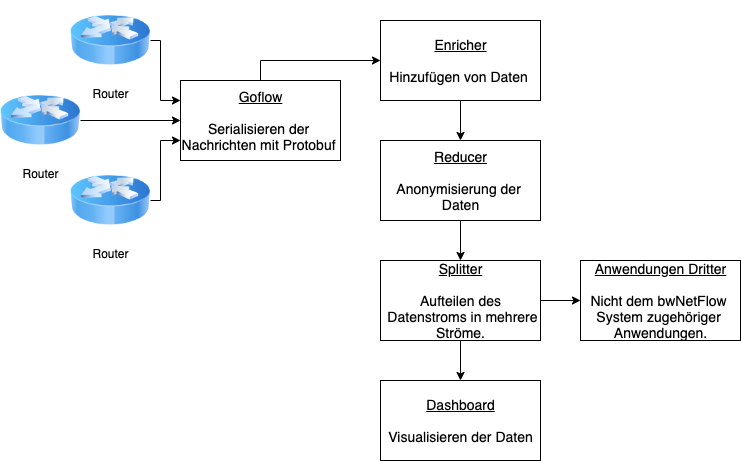
\includegraphics[width=1\textwidth]{images/bwnetflow.png}
    \caption{Die Komponenten des bwNetFlow System}
    \label{fig:bwnetflow}
\end{figure}

Die Komponenten Enricher, Splitter und Reducer sind optional.
Die Ergebnisse können entweder über das Dashboard eingesehen oder von weiteren Customer-Applikationen
weiterverarbeitet werden. 

\subsection{Das Flow Monitoring Protokoll Netflow v9}
Mit Flow Monitoring Protokolle kann Netzwerkverkehr in großen Netzwerkinstallationen beobachtet und analysiert werden \cite{version9flow}.
Anstelle von einzelnen Netzwerkpaketen werden mehrere Pakete einer Verbindung betrachtet.
Informationen über diese zusammengefassten Pakete einer Verbindung werden als Nachricht zur weiteren Analyse versendet.
Diese Nachrichten werden als Flows bezeichnet.
Ein Flow enthält somit Informationen über Pakete einer Verbindung mit fest definiertem Start und Ziel.
\\
Das bwNetFlow System basiert auf dem Flow Monitoring Protokoll Netflow v9 von Cisco.
In dem Netflow v9 Protokoll werden alle Pakete zu einem Flow zusammengefasst, welche die selben Quell-und Zieladressen und Ports haben,
das selbe Vermittlungsschichtprotokoll und Type of Service (Priorisierung von IP-Paketen) benutzen.
Flow Monitoring Pakete enthalten neben allgemeinen Informationen, wie die Göße und Anzahl der beobachteten Pakete auch protokollspezifische Informationen wie TCP Flags. Alle von Netflow v9 erfassten Felder lassen sich in der offiziellen Dokumentation von Cisco einsehen \cite{netflowconfig}.
Bei stark belasteten Knoten kann auch Subsampling betrieben werden. Das heißt, dass Netflow nur eine Teilmenge des Netzwerkverkehrs berücksichtigt.
Die Länge eines Flows, also wieviele Pakete zu einem Flow zusammengefasst werden, kann konfiguriert werden. 
Dies kann auch zeitgesteuert in festen Intervallen passieren.
\\
Viele Netzwerkgeräte wie Switches oder Router unterstützen Flow Monitoring Protokolle. Welche Protokolle im Detail unterstützt werden ist herstellerspezifisch.
Da NetFlow von Cisco entwickelt worden ist, unterstützen die meisten Netzwerkgeräte von Cisco dieses Protokoll.
Aber auch Geräte anderer Hersteller unterstützen oft NetFlow \cite{li2013survey}.
\\
Neben dieser hardwaregebundenen Unterstützung von Flow Monitoring Protokolle gibt es auch reine Softwarelösungen.
Ein Beispiel für eine Softwarelösung ist Flowexport\footnote{\url{https://github.com/cha87de/flowexport}}. Flowexport ist eine auf Containertechnologie (Docker) basierte Lösung.
\\
Die einzelnen Flows von verschiedenen Quellen werden an eine Kollektorkomponente exportiert, welche die Informationen weiter aufbereitet.
In bwNetFlow übernimmt Goflow diese Aufgabe.
Die Quellen, also die Komponenten welche die Netflow Pakete exportieren, müssen die Adresse der Kollektorkomponente kennen.
Netflow ist ein Protokoll der Anwendungsschicht und baut auf dem Transportprotokoll UDP auf \cite{netflowconfig}.

\subsection{Apache Kafka}
Apache Kafka ist eine verteiltes Messaging System und kommt im bwNetFlow System als Middleware zum Einsatz.
Ursprünglich wurde Kafka von Linkedin für die Verarbeitung von Logs großer Verteilter Systeme entwickelt.
Dabei soll der anfallende große Datensatz in Echtzeit verarbeitet werden  \cite{kreps2011kafka}.
\\
Zu herkömmlichen Messaging Systemen grenzt sich Apache Kafka wie folgt ab:
\begin{itemize}
\item Fokus auf Durchsatz statt Konsistenz.
\item Verteiler Einsatz von mehreren Kafka Instanzen anstelle einem Single Point of Failure.
\item Kein Verlust von Performance trotz Anwachsen der persistent zwischengespeicherten Daten.
\end{itemize}
Damit verfolgt Apache Kafka im Vergleich zu anderen Messaging Systemen wie zum Beispiel MQTT\footnote{https://mqtt.org/} andere Ziele. Apache Kafka basiert auf mehreren Komponenten:
\paragraph{Topic:} Container für Nachrichten eines Types.
\paragraph{Broker:} Verschiedene Server auf denen die Nachrichten gespeichert sind. Es gibt kein Masterbroker und damit kein Flaschenhals oder Single Point of Failure. Topics können für bessere Ausfallsicherheit auf unterschiedlichen Brokern repliziert werden. Der Replikationsfaktor, also wie viele Replikate einer Topic erzeugt werden sollen, ist frei konfigurierbar. 
\paragraph{Partition:} Topics werden in mehrere Partitionen aufgeteilt. Die Partitionen sind wiederum auf die Broker aufgeteilt. Durch Partitionen wird Lastbalancierung und Parallelisierung realisiert. Innerhalb einer Partition ist die Reihenfolge der Nachrichten garantiert, aber nicht Partitionsübergreifend.  
\paragraph{Producer:} Diese Komponenten fügen Nachrichten in Topics ein. Mehrere Producer können Nachrichten in eine Partition schreiben. In welche Partition geschrieben wird, wird entweder über einen optionalen Schlüssel oder über ein Round Robin Scheduler bestimmt. Nachrichten die in Apache Kafka eingefügt werden, werden persistiert.
\paragraph{Consumer:} Die Consumer sind das Gegenstück zu den Producern. Die Consumer lessen Nachrichten aus den Topics. Beim Lesen werden Nachrichten in den Topics nicht gelöscht. Stattdessen wird ein Zeiger erhöht, welcher auf die zu letzt gelesene Nachricht zeigt. Dieser Zeiger wird Offset genannt. Pro Partition kann nur ein Consumer Nachrichten auslesen. Aber ein Consumer kann gleichzeitig auf mehrere Partitionen lesend zugreifen.
\paragraph{Consumer Group:} Mehrere Consumer, welche auf die selbe Topic zugreifen wollen, werden zu einer Consumer Group zusammengefasst. Jedem Consumer wird mindestens eine Partition zugewiesen und die Nachrichten in einer Topic, somit auf die Consumer verteilt. Allerdings kann auf eine Partition maximal ein Consumer gleichzeitig zugreifen. Wenn Consumer hinzugefügt werden oder nicht mehr verfügbar sind, wird die Zuteilung von Consumer und Partition neu bestimmt. Dieses Verfahren wird Rebalancing genannt. Apache Kafka garantiert At Least Once Delivery. Die Anzahl der Consumer in einer Consumer Group kann nicht höher als die Anzahl der Partitionen der Topic sein.
\\
\begin{figure}[H]
    \centering
    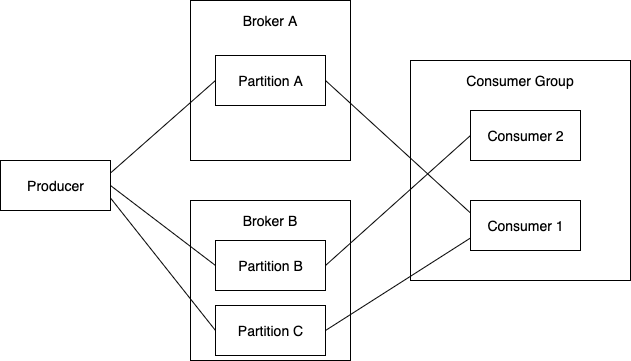
\includegraphics[width=0.8\textwidth]{images/kafka.png}
    \caption{Architektur eines Kafka Clusters mit einer Topic}
    \label{fig:kafkaarchitecture}
\end{figure}

Kafka schreibt kein Dateiformat für die Nachrichten vor. Das Dateiformat ist frei wählbar.
Bei bwNetFlow werden Nachrichten mit Protocol Buffers (Protobuf) Bibliothek serialisiert und in diesem Binärem Format in eine Topic geschrieben.
Apache Kafka ist abhängig von Apache Zookeeper. Zookeeper verwaltet den Offset Zeiger, initiiert Rebalancing und verwaltet Broker, Consumer und Producer \cite{kreps2011kafka}.


\section{Gescheiterter Ansatz: Alternative Flow Monitoring Protokolle}
In diesem Ansatz sollen alle notwendigen Informationen über das Flow Monitoring Protokoll bezogen werden.
Die Steuerinformationen von Multipath TCP sind in TCP Optionen kodiert.
Folglich wird an das Flow Monitoring Protokoll die Voraussetzung gestellt, TCP Optionen exportieren zu können.
NetFlow v9 exportiert allerdings keine TCP Optionen. 
Um diese Limitierung zu umgehen werden alternative Flow Monitoring Protokolle betrachtet. 
Der von bwNetFlow verwendete Flow Monitoring Collector Goflow, unterstützt neben NetFlow v9 auch sFlow \cite{li2013survey, phaal2001rfc3176} und IPFIX (IP Flow Information Export) \cite{li2013survey, claise2013specification}.
\\
NetFlow ist ein proprietäres Format von Cisco. IPFIX ist ein offenes, von der IETF standardisiertes Protokoll, welches auf NetFlow basiert. 
Aufgrund dieser Beziehung sind sich beide Protokolle sehr ähnlich.
Die Internet Assigned Numbers Authority (IANA) hat alle unterstützten Felder aufgelistet\footnote{\url{https://www.iana.org/assignments/ipfix/ipfix.xml}}.
Aus dieser Liste ist eine Unterstützung von TCP Options zu entnehmen.
Exportiert werden dabei die standardisierte Nummern der gesetzten TCP Optionen.
Damit wäre Flow Monitoring mit IPFIX eine Möglichkeit Informationen über Multipath TCP zu erlangen.
\\
In einem einfachen Versuchsaufbau soll IPFIX genauer hinsichtlich dem Export von TCP Optionen untersucht werden.
Da flowexport IPFIX nicht unterstützt, muss dazu eine Alternative gefunden werden.
In einer Ubuntu Virtuellen Maschine wird der gesamte Netzwerkverkehr über einen Open Virtual Switch (Open vSwitch) \cite{pfaff2015design} geleitet.
Open vSwitch ist ein rein virtueller Switch. Dadurch lässt ein Open vSwitch sich passend zum Anwendungsfall konfigurieren.
Open vSwitch unterstützt auch das erforderliche IPFIX Protokoll. 
Auf der Virtuellen Maschine ist ein Linux Kernel mit Multipath TCP Patch installiert.
Auf dem Host System ist Goflow installiert. Der virtuelle Switch sendet IPFIX Pakete an Goflow. 
Für dieses Experiment wurde Goflow so modifiziert, dass die empfangenen IPFIX Pakete auf stdout ausgegeben werden.
Zusätzlich werden mit Wireshark die IPFIX Pakete manuell abgehört.
Aus der Virtuellen Maschine wird eine Multipath TCP Testwebsite\footnote{\url{http://www.amiusingmptcp.de}} über cURL aufgerufen.
 
\begin{figure}[H]
    \centering
    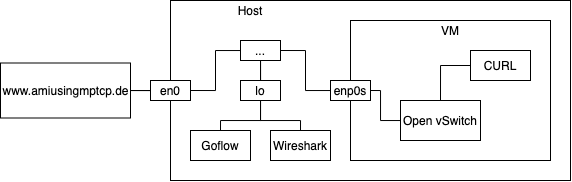
\includegraphics[width=1\textwidth]{images/flowmonitoringmptcp.png}
    \caption{Versuchsaufbau - Multipath TCP Monitoring über herkömmliche Flow Monitoring Protokolle}
    \label{fig:flowmonitoringmptcp}
\end{figure}

Überraschend sind in der Ausgabe keine Informationen über TCP Options enthalten.
Das Verhalten lies sich nach erneutem Lesen des RFC 7011 erklären.
Viele Felder, unter anderem das TCP Options Feld, sind in IPFIX optional.
\\
Dies ist problematisch, da die Funktionsweise von Multipath TCP Monitoring unter IPFIX stark von der Netzwerkhardware, beziehungsweise eingesetzter Software abhängig ist.
Darüber hinaus ist mit diesem Ansatz eine weitere Analyse des Multipath TCP Verkehres schwierig. Es werden die Nummern der beobachteten TCP Optionen exportiert, aber nicht die Nachrichten.  
\\
Über das sFlow Protokoll lässt sich nicht auf die TCP Options zugreifen \cite{phaal2001rfc3176}. Damit eignet sich dieses Protokoll nicht um Multipath TCP zu überwachen.
\\
Beide alternative Netzwerkprotokolle eignen sich nicht um Multipath TCP Ströme zu überwachen.
Somit eignen sich weder Netflow v9, IPFIX noch sFlow, um das bwNetFlow System um die Unterstützung von Multipath TCP zu erweitern.
Der Ansatz, alternative Flow Monitoring Protokolle zu verwenden, ist damit gescheitert.

\section{Zweiter Ansatz: MPTCP Sniffer und MPTCP Aggregator}
Da das Beschaffen der Multipath TCP Optionen über herkömmliche Flow Monitoring Protokolle gescheitert ist, müssen alternative Quellen gefunden werden.
Diese Informationen aus alternativen Quellen müssen dann mit den Daten aus dem herkömmlichen Flow Monitoring verknüpft werden. 
Es werden mit dem MPTCP Sniffer und dem MPTCP Aggregator zwei neue Komponenten eingeführt um dieses Ziel zu erreichen.
Zur Vereinfachung werden die bwNetFlow Komponenten Splitter und Reducer im folgenden Abschnitt nicht weiter betrachtet.
Diese Komponenten können aber ohne große Änderungen auch in dem vorgestelltem Ansatz verwendet werden.

\begin{figure}[H]
    \centering
    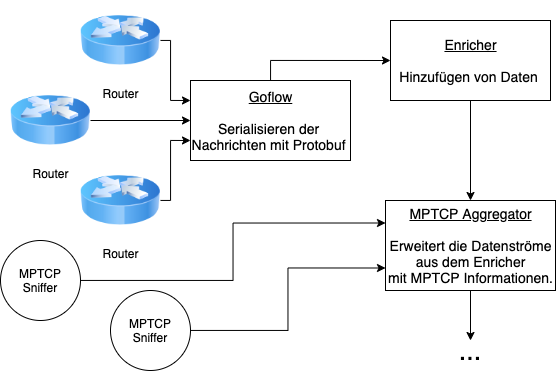
\includegraphics[width=0.8\textwidth]{images/extendedbwnetflow.png}
    \caption{Systemarchitektur des zweiten Ansatz um bwNetFlow mit Multipath TCP Informationen zu erweitern.}
    \label{fig:sniffer_component}
\end{figure}

\subsection{MPTCP Sniffer}
Die MPTCP Sniffer\footnote{https://github.com/Multipath-TCP-bwNetFlow/MPTCP-Sniffer} Komponente hört den Netzwerkverkehr ab und extrahiert Pakete mit Multipath TCP Optionen.
Diese Pakete werden analog zu Flow Monitoring Protokolle, in Flows zusammengefasst.
Danach werden die Flows in eine dedizierte Kafka Topic geschrieben.
\\
Der MPTCP Sniffer setzt sich aus drei Modulen zusammen: dem Sniffer, der Batch Processor Komponenten und dem Kafka Producer.

\begin{figure}[H]
    \centering
    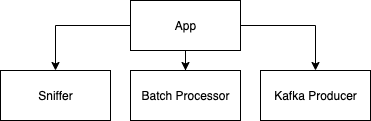
\includegraphics[width=0.6\textwidth]{images/sniffer_component.png}
    \caption{Komponenten des MPTCP Sniffers}
    \label{fig:sniffer_component}
\end{figure}

Der Sniffer basiert auf der gopacket\footnote{\url{https://github.com/google/gopacket}} Bibliothek von Google. Diese baut wiederum auf pcap auf. Die pcap Bibliothek kümmert sich um das Abhören von Netzwerkpaketen \cite{manpcap}. Gopacket stellt weitere Werkzeuge zur Analyse der empfangenen Pakete bereit. Es werden im weiteren Verlauf nur TCP Pakete betrachtet bei welchen Multipath TCP Optionen gesetzt sind. Alle anderen empfangene Pakete werden sofort verworfen.
\\
Die Batch Komponente wandelt die einzelnen Pakete in ein Flow um. Ähnlich wie bei Netflow v9 werden Pakete in einem bestimmten Zeitraum gesammelt und alle Pakete mit gleicher Quelle und Ziel zu einem Flow Paket zusammengefasst. Dabei werden die Quell-und Ziel IP Adressen und die Ports analysiert. Der Zeitraum über den sich ein Flow erstreckt, kann konfiguriert werden. Die Attribute eines Flow Pakets sind in der Tabelle \ref{tbl:mptcp_fields} einsehbar. 

\begin{figure}[H]
\begin{center}
    \begin{tabular}{ | l | p{5cm} |}
    \hline
    \textbf{Attribut} & \textbf{Beschreibung}  \\ \hline
    timestampCaptured & Zeitpunkt, wann das erste Paket des Streams  erfasst wurde.\\ \hline
    srcAddr & Quelladresse aller Pakete im Flow.\\ \hline
    dstAddr & Zieladdresse aller Pakete im Flow.   \\ \hline
    srcPort & Quellport aller Pakete im Flow.   \\ \hline
    dstPort & Zielport aller Pakete im Flow   \\ \hline
    mptcpOptions & Alle Multipath TCP Optionen die in den Paketen des Flows erfasst werden.  \\ \hline
    \end{tabular}
\end{center}    
\caption{TCP Optionen zur Steuerung von Multipath TCP}
\label{tbl:mptcp_fields}
\end{figure}

Der Producer schreibt die Flow Pakete in eine dedizierte Kafka Topic. Die Pakete werden mit der Protocol Buffers Bibliothek serialisiert.
Der Producer verwendet eine modifizierte Version des bwNetFlows Kafka Connector. 
Eine Modifikation ist notwendig, da der orginale Kafka Connector stark an das von Goflow festgelegte Nachrichtenformat gekoppelt ist.
Dieses Nachrichtenformat muss an das der Flow Pakete angepasst werden.
Außerdem wurde der Kafka Connector um eine Fehlerbehandlung beim Schreiben in eine Kafka Topic ergänzt.
\\
Der MPTCP Sniffer basiert technisch auf der selben Platform wie die vorhandenen Komponenten des bwNetFlow System: als Programmiersprache kommt Go zum Einsatz.

\subsection{MPTCP Aggregator}
Der Multipath TCP Aggregator\footnote{\url{https://github.com/Multipath-TCP-bwNetFlow/MPTCP-Aggregator}} ist für das Zusammenführen der Nachrichten des Flow Monitorings vom bwNetFlow Projekt und der neuen MPTCP Flow Pakete vom MPTCP Sniffer zuständig. Der MPTCP Aggregator liest die Ausgangsinformationen aus der jeweiligen Topic und schreibt das zusammengefügte Ergebnis in eine weitere Topic.
Drei nichtfunktionale Anforderungen ergeben sich:
\begin{itemize}
\item Beim Flow Monitoring kann die zu verarbeitende Datenmenge sehr groß werden. Daher muss der MPTCP Aggregator sehr gut mit steigender Anzahl ankommender Nachrichten skalieren.
\item Die Lösung muss einfach in ein existierendes Kafka basiertes System integrierbar sein.
\item Die Zusammenführung der Daten soll möglichst in Echtzeit stattfinden. Es soll vermieden werden, dass sich die Latenz des Systems stark erhöht.
\end{itemize}

Um diese nichtfunktionalen Anforderungen zu erfüllen, gibt es Lösungen aus dem Big Data Bereich.
Es gibt drei grundlegende Ansätze um große Datenmengen zu verarbeiten: Batch Processing, Micro Batch Processing und Stream Processing.
Batch Processing eignet sich eher für das Analysieren von großen, statischen Datensätzen. Außerdem ist Batch Processing nicht echtzeitfähig. 
Micro Batch Processing ist Echtzeitfähiger als Batch Processing. Stream Processing Systeme ermöglichen tendenziell die geringste Latenz. Dies wird allerdings mit einem höheren Aufwand für Fehlertoleranz erkauft.
Wenn die Bearbeitung eines Datensatzes gegenüber einem Client bestätigt werden soll, reicht es bei (Micro) Batch Processing Systemen aus, für jeden abgearbeiteten Batch eine Bestätigung zu generieren. Bei Stream Processing muss jede Nachricht einzeln bestätigt werden \cite{lopez2016performance}. 
Bei einem Flow Monitoring Werkzeug müssen keine harte Anforderungen an die Konsistenz erfüllt werden. Alleine durch mögliches Sampling durch die Netzwerkkomponenten und Sniffer, welche den Verkehr beobachten, werden nicht alle Flows erfasst.
Zu den geforderten nichtfunktionalen Anforderungen passt Stream Processing am besten.
\\
Apache Kafka bietet die Basis um ein Stream Processing System zu bauen. 
Stream Processing Systeme lassen sich allgemein in fünf Komponenten unterteilen \cite{isah2019survey}:
 
\begin{itemize}
\item Data Stream Ingestion Layer: Zuführen der Daten von der Quelle an den Stream Processing Layer. 
\item Data Stream Processing Layer: Hier werden die Daten verarbeitet. Dabei stehen zustandslose und zustandsorientierte Funktionen bereit. Analog zu Queries in relationalen Datenbanken können Anfragen und Join Operationen auf einen oder mehrere Datenströme durchgeführt werden. Dafür werden Abschnitte von einem oder mehreren Datenströmen betrachtet (Window Operationen wie z.b. Sliding Windows).
\item Storage Layer: Bei statusbehafteten Operationen im Stream Processing Layer müssen Daten zwischengespeichert werden. Dies wird vom Storage Layer durchgeführt.
\item Ressource Management Layer: Verwaltung der Streaming Platform. Bei Kafka basierten Systemen wird diese Rolle von Zookeeper eingenommen. 
\item Output Layer: Zuführen der gewonnenen Daten zu weiteren Anwendungen (zum Beispiel ein Dasboard). 
\end{itemize}
Der  Data Stream Ingestion Layer, Output Layer und Storage Layer sind durch Apache Kafka realisierbar. Der Ressource Management Layer ist in Apache Kafka durch Zookeeper realisiert. Für ein vollständiges Stream Processing System muss nur noch der Data Stream Processing Layer realisiert werden.
 \\
Apache Kafka liefert mit Kafka Streams einen Stream Processor mit. Verfügbar ist dieser in dem Apache Kafka Java SDK.
Es sind keine weiteren Abhängigkeiten erforderlich und eine einfache Integration in eine bestehende, auf Kafka basierende Architektur, ist gewährleistet.
Außerdem zeichnet sich Kafka Streams durch seine Einfachheit und leichte Erlernbarkeit aus.
Kafka Streams Anwendungen lassen sich über zwei APIs programmieren. Die abstraktere Kafka Streams API ermöglicht statuslose Operationen (zum Beispiel map oder filter) und statusbehaftete Operationen, wie das Zusammenführen mehrerer Datenströme (join oder aggregation).
Der eher im low level Bereich angesiedelte Processor API ermöglicht eine direkte Interaktion mit dem Storage Layer. Im Gegensatz zu der Stream API wird nicht mit einem abstrakten Datenstrom interagiert, sondern mit einer Datenstruktur, welche Schlüssel auf einen Wert abbilden \cite{kafkastreams}. 
\\
Der MPTCP Aggregator integriert die Flow Information mit den MPTCP Daten in zwei Schritten:
\begin{enumerate}
\item Über eine Left Join Operation werden die MPTCP Informationen mit den Flow Informationen verknüpft. Alle zueinander passenden Informationen, die in einem zeitlich konfigurierbaren Fenster auftreten, werden miteinander verknüpft. Diese Operation lässt sich mit der High Level Kafka Streams DSL umsetzen.
\item Aufgrund der Charakteristik von Left Join ergeben sich Duplikate. Wenn die Multipath TCP Information nach der Flow Information eintrifft, ergeben sich zwei Ergebnisse. Das erste Ergebnis enthält nur die Flow Information, das zweite Ergebnis enthält neben der Flow Information auch die MPTCP Information. Die Semantik der Left Join Operation ist in Abbildung \ref{fig:leftjoinsemantics} dargestellt. Daher muss in diesem Schritt das erste Ergebnis entfernt werden, wenn eine Multipath TCP Information vorliegt. Dieser Schritt lässt sich mit der Processor API implementieren.
\end{enumerate}

\begin{figure}[H]
    \centering
    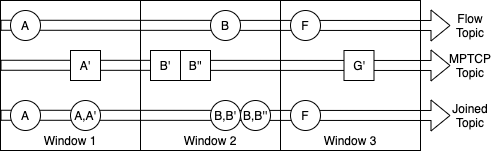
\includegraphics[width=0.9\textwidth]{images/leftjoinsemantic.png}
    \caption{Left Join Semantik in Kafka Streams}
    \label{fig:leftjoinsemantics}
\end{figure}

Die MPTCP Aggregator Anwendung ist in Java implementiert.
Die wichtigsten Klassen sind:

\paragraph{Aggregator:} Der Aggregator führt die Left Join Operation durch und speichert die Ergebnisse in eine temporäre Topic.

\paragraph{DeduplicationProcessor:} Der Deduplication Processor liest die Nachrichten aus der temporären Topic aus und entfernt die Duplikate, die durch das Left Join Verfahren entstehen.

\paragraph{CLIConfigurator:} Ermöglicht das Konfigurieren der Anwendung über Flags. Zum Beispiel kann die Größe des Window beim Left Join eingestellt werden. 

\paragraph{KafkaStreamsAppBuilder und TopologyDescriptor:} Kleines Framework um eine Streamingtopology bestehend aus High Level (Java Kafka DSL) und Low Level (Kafka Processor API) aufzubauen.

\paragraph{KafkaProtobufSerde:} Hilfsklasse um die ankommenden Protobuf Nachrichten in Objekte zu deserialisieren und Java Nachrichtenobjekte in Protobuf Nachrichten zu serialisieren.
\\
\\
Zusätzlich kann eine Whitelist konfiguriert werden. Dadurch werden nur Flows mit bestimmten IP Adressen und Ports weiter berücksichtigt.


\section{Deployment in der bwCloud}
Die Baden-Württemberg Cloud (bwCloud) stellt Cloud Computing Dienste für Lehr-und Forschungseinrichtungen in Baden-Württemberg bereit \cite{bwcloud}.
Technisch basiert die bwCloud auf OpenStack. 
OpenStack ist eine Infrastructure as a Service Platform. Über OpenStack lassen sich unter anderem virtuelle Maschinen und virtuelle Netzwerke einrichten \cite{rosado2014overview}.
Um das modifizierte bwNetFlow System in einer verteilten Installation zu testen wird es in der bwCloud deployt.
\\
Mit Ausnahme des MPTCP Sniffers werden alle Komponenten in Docker Container ausgeliefert.
Verwaltet werden die Container mit der GitHub Container Registry (ghcr.io). 
Die Komponenten Flowexport (Netzwerksniffer, welcher den Export von Netflow v9 Nachrichten unterstützt) und der MPTCP Sniffer werden auf den einzelnen virtuellen Maschinen installiert, auf denen der Netzwerkverkehr analysiert werden soll. 
In der Abbildung \ref{fig:deployment_bwCloud} sind dies die Virtuellen Maschinen VM 2 und VM 3.
Die virtuellen Maschinen VM2 und VM3 sind jeweils an zwei von einander getrennte, Netzwerke angebunden.
Damit können zwei Multipath TCP Subflows zwischen den Maschinen aufgebaut werden. 
\\
Alle anderen Komponenten Kafka, Zookeeper, Enricher, Goflow und der MPTCP-Aggregator, können automatisiert über eine Docker Compose Datei\footnote{\url{https://github.com/Multipath-TCP-bwNetFlow/mptcp-bwNetFlow}} bereitgestellt werden. Diese Komponenten werden auf der Virtuellen Maschine VM 1 installiert.
Netzwerkverkehr wird über iperf3\footnote{https://iperf.fr/} erzeugt.
Ein Beispiel eines Netflow v9 Paketes, dem Ergebnis des MPTCP Sniffers und das Ergebnis des MPTCP Aggregator befindet sich im Anhang.

\begin{figure}[H]
    \centering
    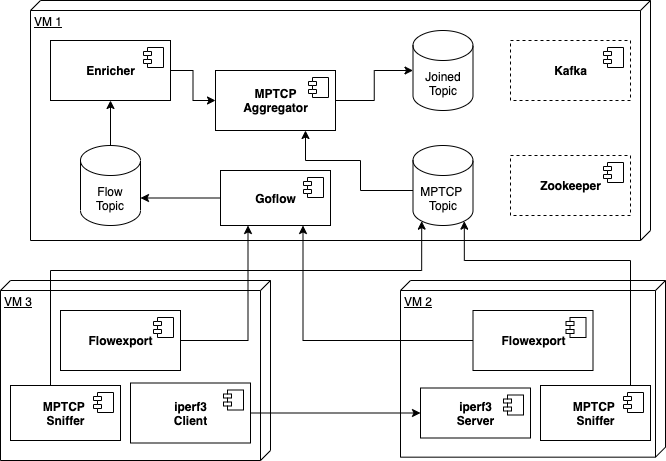
\includegraphics[width=0.9\textwidth]{images/deployment_bwCloud.png}
    \caption{Deployment des modifizierten bwNetFlow Systems in der bwCloud}
    \label{fig:deployment_bwCloud}
\end{figure}

Beim erstmaligen Deployment auf die bwCloud ist das Problem aufgetreten, dass der MPTCP Sniffer keine Nachrichten nach Kafka schreiben konnte.
Dieses Problem lässt sich mit der Funktionsweise, wie Consumer und Producer sich mit einem Broker verbinden, erklären.
Eine Voraussetzung für das Verbinden ist, dass die Consumer und Producer die Adresse des Brokers kennen.
Falls mehrere Broker existieren, genügt es wenn die Adresse eines Brokers bekannt ist.
Der Verbindungsvorgang läuft in folgenden Schritten ab:
\begin{enumerate}
\item Zuerst sendet der Producer oder Consumer eine Anfrage an einen Broker.
\item Der Broker gibt daraufhin die Adressen aller Broker im System zurück.
\item Der Producer oder Consumer wählt aus der Liste aller Broker den passenden Broker aus. Der passende Broker ist der Broker mit der Partition auf die der Producer oder Consumer
zugreifen will.
\end{enumerate}
Somit muss der Producer oder Consumer den Broker, auf welchem die benötigte Partition gespeichert ist, selbst herausfinden.
Der indirekte Verbindungsvorgang sorgt dafür, dass dem Producer oder Consumer alle verfügbaren Broker bekannt gemacht werden und gleichzeitig initial nur eine Adresse eines Brokers bekannt sein muss. 
Beim verteilten Deployment in der bwCloud gibt der Broker allerdings die falsche Adresse zurück.
Auf dem lokalen Entwicklungsaufbau kommt dieses Problem nicht vor. Erst mit verteilten Deployment ist der Fehler aufgetreten.  
Es wird nicht die Adresse zurückgegeben mit welcher der Broker von anderen Servern erreichbar ist. 
Durch Konfiguration von Kafka über ein spezielles Flag, wie in Listing \ref{listing:advertised_listener} kann das Problem behoben werden.
Durch die Konfiguration bekommen Clients (Producer oder Consumer), welche auf anderen Servern bereitgestellt sind, die IP Adresse 193.196.38.1 zurückgeliefert. Lokale Clients bekommen die Adresse des Docker Netzwerkes.  

\begin{figure}[H]
\begin{lstlisting}
 KAFKA_CFG_ADVERTISED_LISTENERS=CLIENT://kafka:9092,EXTERNAL://193.196.38.1:9093 
\end{lstlisting}
\caption{Konfiguration welche IP Adresse vom Kafka Broker an den Client zurückgegeben werden soll.}
\label{listing:advertised_listener}
\end{figure}


\section{Fazit}
Das bwNetFlow System ist ein Monitoring Tool für große Netzwerke.
In dieser Arbeit wird bwNetFlow um die Möglichkeit, das Multipath TCP Protokoll zu verarbeiten, erweitert.
Die Steuerinformationen von Multipath TCP werden in TCP Optionen kodiert. 
Es werden zwei verschiedene Ansätze betrachtet:
Die Idee im ersten Ansatz liegt darin, herkömmliche Flow Monitoring Protokolle zu benutzen, um TCP Optionen zu erfassen.
Alle in dieser Arbeit betrachteten Flow Monitoring Protokolle unterstützten das Mitschneiden von TCP Optionen nicht oder boten dies nur als Optionales Feature an.
Dadurch ist dieser Ansatz praktisch nicht umsetzbar.
Im zweiten Ansatz werden im bwNetFlow System weitere Komponenten eingeführt: den MPTCP Sniffer und den MPTCP Aggregator.
Der MPTCP Sniffer sammelt alle TCP Pakete mit Multipath TCP Optionen und fasst zu einer Verbindung zusammengehörige Pakete zu einem Flow zusammen.
Der MPTCP Aggregator fügt diese MPTCP Flows mit den Flows aus dem bwNetFlow System zusammen und beseitigt technisch bedingte Duplikate.
Damit ist eine Unterstützung von Multipath TCP im bwNetFlow System gewährleistet.
\\
Neben der Entwicklung der zwei neuen Komponenten wurde das System in der bwCloud testweise auf drei Virtuellen Maschinen installiert.
Dadurch kann der Betrieb als verteiltes System erprobt werden und Probleme, welche sich durch die Verteilung der Komponenten ergeben, behoben werden.
\\
Die Arbeit legt den Grundstein um Multipath TCP Ströme, in einem großen Netzwerk weiter zu Analysieren.


\section{Ausblick}

\subsection{Sampling}
Beim Monitoring großer Netzwerke werden die Netflow Exporter meist so konfiguriert, dass nur manche Pakete erfasst werden.
Dieses Verfahren wird als Sampling bezeichnet.
Die Samplingrate kann frei konfiguriert werden.
Das bwNetFlow System wurde mit einer Samplingrate von 1/32 produktiv gesetzt\footnote{https://github.com/bwNetFlow/bwNetFlow}.
\\
Wenn auch bei den  Multipath TCP Sniffern Sampling zum Einsatz kommen soll, ist dies problematisch.
Es finden bei kleinen Samplingraten wenige Zuordnungen von Flows aus dem bwNetFlow System zu Multipath TCP Flows aus dem MPTCP Sniffer statt.
Eine optimale Lösung wäre, wenn an den MPTCP Sniffern kein Sampling zum Einsatz kommt.
Dabei kann zu jedem gesampeltem Flow ein Multipath TCP Flow zugeordnet werden.
\\\
Um die Machbarkeit der optimalen Lösung zu bestimmen, müssen Lasttests durchgeführt werden. 
Bei zu geringer Performance kann dann auch auf Seiten der MPTCP Sniffer gesampelt werden.
Je geringer die Samplingrate auf Seiten des MPTCP Sniffers, umso geringer ist die Wahrscheinlichkeit, dass sich passende Flows treffen. 
Es wird die Qualität der Ergebnisse gegen Performance getauscht.


\subsection{Erweitern des MPTCP Sniffers}
Zurzeit extrahiert der MPTCP Sniffer nur welche Multipath TCP spezifische TCP Optionen gesetzt sind.
Um weitere Analysen durchzuführen ist dies nicht ausreichend. 
Zum Beispiel wird bei der Add Address TCP Option auch eine Address ID und die letztendlich neue IP-Adresse mitgesendet:
\begin{figure}[H]
\begin{lstlisting}
    Multipath Transmission Control Protocol: Add Address
        Kind: Multipath TCP (30)
        Length: 8
        0011 .... = Multipath TCP subtype: Add Address (3)
        .... 0100 = IP version: 4
        Address ID: 3
        Advertised IPv4 Address: 10.0.1.2
\end{lstlisting}
\caption{Add Address TCP Option}
\end{figure}

Analog verhält es sich mit den anderen Multipath TCP Optionen.
Die MPTCP Sniffer Komponenten muss erweitert werden, dass auch diese zusätzlichen Informationen erfasst werden.
Bei Erweiterung des Sniffers müssen auch die Protobuf Definitionen angepasst werden, um die neu gewonnenen Informationen in MPTCP Flows weitergeben zu können.

\subsection{bwNetFlow Komponenten anpassen}

Andere bwNetFlow Komponenten, welche hinter den MPTCP Aggregator geschaltet werden, müssen auch leicht modifiziert werden.
Dies sind zum Beispiel der Reducer oder der Splitter.
Da im Protobuf Format neue Multipath TCP spezifische Felder hinzugefügt wurden, 
können die schon vorhandenen Komponenten die Nachrichten nicht mehr deserialisieren.
Für in Go programmierte Anwendungen seht eine entsprechend generiertes Go Datei bereit\footnote{\url{https://github.com/Multipath-TCP-bwNetFlow/mptcp-flow-protobuf}}.

\subsection{Weitere Automatisierung des Deployments}
Durch eine Docker Compose Datei lässt sich das modifizierte bwNetFlow System weitestgehend automatisch deployen.
Allerdings gibt es noch ein Schritt der manuell ausgeführt werden muss:
Die Topics müssen noch manuell erzeugt werden.
Auf einer Shell des Apache Kafka Containers müssen die Befehle im Listing \ref{listing:topics} ausgeführt werden.
Ideal wäre, wenn dieser Schritt auch automatisiert ablaufen könnte.

\begin{figure}[H]
\begin{lstlisting}
/opt/bitnami/kafka/bin/kafka-topics.sh --create --zookeeper zookeeper:2181 --replication-factor 1 --partitions 1 --topic mptcp-bwnetflow-aggregator-output
/opt/bitnami/kafka/bin/kafka-topics.sh --create --zookeeper zookeeper:2181 --replication-factor 1 --partitions 1 --topic mptcp-packets
/opt/bitnami/kafka/bin/kafka-topics.sh --create --zookeeper zookeeper:2181 --replication-factor 1 --partitions 1 --topic mptcp-joined
/opt/bitnami/kafka/bin/kafka-topics.sh --create --zookeeper zookeeper:2181 --replication-factor 1 --partitions 1 --topic flows-enriched
\end{lstlisting}
\caption{Befehle um Topics zu erstellen}
\label{listing:topics}
\end{figure}

\subsection{Weitere Analysen}
Die gewonnen Rohdaten können weiter analysiert werden.
Dafür können neue Komponenten in das System eingefügt werden.
Beispielsweise kann ermittelt werden, wieviele der TCP Verbindungen Multipath TCP Verbindungen sind,
aus wie vielen Subflows eine logische Verbindung besteht oder wieviele Clients im Schnitt Multipath TCP fähig sind.
\\
Das bwNetFlow System enthält ein Dashboard, um die erfassten Daten zu visualisieren.
Dies kann erweitert werden um die durch weitere Analysen gewonnenen Daten zu visualisieren.

\newpage

\bibliographystyle{unsrt}
\bibliography{quellen}
%\printbibliography

\newpage

\section{Anhang}
\subsection{Beispiel der Nachrichten}

\begin{figure}[H]
\begin{lstlisting}
timestampCaptured:1614446288
srcAddr:193.196.37.204
mptcpOptions:[DSS, ADD_ADDR, MP_CAPABLE]
dstPort:55092
seqNum:1864576622
dstAddr:193.196.38.233
srcPort:5201
\end{lstlisting}
\caption{Nachrichten aus dem MPTCP Sniffer}
\end{figure}

\begin{figure}[H]
\begin{lstlisting}
SrcPort:5201
SrcAddr:193.196.37.204
DstPort:55092
TimeReceived:1614446415
SequenceNum:78
DstAddr:193.196.38.233
Bytes:455320
Type:NETFLOW_V9
TCPFlags:22
Proto:6
Packets:7588
ProtoName:TCP
SamplerAddress:193.196.38.233
SrcMac:274973441647955
Etype:2048
\end{lstlisting}
\caption{Flow aus dem beNetFlow Enricher}
\end{figure}

\begin{figure}[H]
\begin{lstlisting}
SrcPort:5201
isMPTCPFlow:true
SrcAddr:193.196.37.204
DstPort:55092
TimeReceived:1614446415
SequenceNum:78
DstAddr:193.196.38.233
Bytes:455320
Type:NETFLOW_V9
TCPFlags:22
mptcpOptions:[DSS, ADD_ADDR, MP_CAPABLE]
Proto:6
Packets:7588
ProtoName:TCP
SamplerAddress:193.196.38.233
SrcMac:274973441647955
Etype:2048
\end{lstlisting}
\caption{Zusammengefügter Flow}
\end{figure}

\end{document}